% Proposed problem for ACM-ICPC, PacNW region, 2012
% Kent Jones

\documentclass{article}
\usepackage{verbatim}
\usepackage{graphicx}
\usepackage{tabularx}
\usepackage{wrapfig}
\title{ Rings and Runes }
% Alter some LaTeX defaults for better treatment of figures:
% See p.105 of "TeX Unbound" for suggested values.
% See pp. 199-200 of Lamport's "LaTeX" book for details.
%   General parameters, for ALL pages:
\renewcommand{\topfraction}{0.9}	% max fraction of floats at top
\renewcommand{\bottomfraction}{0.8}	% max fraction of floats at bottom
%   Parameters for TEXT pages (not float pages):
\setcounter{topnumber}{2}
\setcounter{bottomnumber}{2}
\setcounter{totalnumber}{4}     % 2 may work better
\setcounter{dbltopnumber}{2}    % for 2-column pages
\renewcommand{\dbltopfraction}{0.9}	% fit big float above 2-col. text
\renewcommand{\textfraction}{0.07}	% allow minimal text w. figs
%   Parameters for FLOAT pages (not text pages):
\renewcommand{\floatpagefraction}{0.7}	% require fuller float pages
% N.B.: floatpagefraction MUST be less than topfraction !!
\renewcommand{\dblfloatpagefraction}{0.7}	% require fuller float pages

\begin{document}
\date{}
\maketitle

\section{Description}

\begin{wrapfigure}{r}{6cm}
\vspace{-12pt}
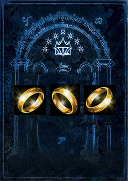
\includegraphics[width=4cm]{RunesAndRings}
\centering
\caption{A gate in the Mines of Moria that is controlled by an ancient Rune}
\vspace{-12pt}
\end{wrapfigure}
Frodo has entered the mines of Moria and encountered a series of gates.  Each gate has written upon it an ancient riddle describing the state of a set of special rings which control that particular gate. By examining the riddle, Frodo can determine whether or not the gate can be opened, or if it is simply a death trap.

\textbf{Riddles} consist of multiple \textbf{runes}. A valid \textbf{rune} contains exactly \textbf{3 statements} about 3 different \textbf{rings}. Each \textbf{statement} in a rune is either \textbf{true} or \textbf{false}, depending on the \textbf{state} (spinning or not spinning) of a specific ring in the set of rings controlling the gate. The riddle for a particular gate does not have to use all of the possible rings contained in the gate's controlling set.

To open the gates, the hobbits must read the riddle, then, decide which of the rings to spin, and which of the rings to leave alone. Once they have the correct rings spinning, they say an incantation, and if the entire riddle for the gate is satisfied the gate will open. For the gate to open, every rune in the riddle must have \textbf{at least} one statement in it that is true. %based on the state of the set of rings $(3 \le rings \le 22)$ located outside of a gate. 

For example, consider a specific rune: \verb+1 -2 3 0+.  This rune will be true if (ring 1 is spinning) \textbf{OR} (ring 2 is NOT spinning) \textbf{OR} (ring 3 is spinning).  (NOTE: The \verb+0+ indicates the end of a rune, and at least one of the statements in that rune must be true for that specific rune to be true.) If a ring number in a rune is negative (e.g., \verb+-2+), it means that ring 2 must NOT be spinning for that particular statement in the rune to be true.  If the ring number is positive, (e.g., \verb+3+) it means that ring 3 MUST be spinning for that statement in the rune to be true.  A specific ring may only appear one time in a specific rune, however, a ring may be used multiple times in the entire riddle, just not in the same rune!

\section{Input}

The input will consist of the following:
\begin{itemize}

\item The first line of input contains a single integer $g$ (where $1 \le g \le
30$), which denotes the number of gates with riddles to be decoded.

\item The first line for each gate contains two integers, $rings$ (where $3 \le
rings \le 22$) and $runes$ (where $1 \le runes \le 100$), separated by a space.
$rings$ is the number of rings in the controlling set; each ring is numbered
from 1 to $rings$, and riddles are not required to use every possible ring.
$runes$ is the number of runes that must be satisfied by the set of $rings$.

\item The next $runes$ lines describe individual runes that specify the
relationships between the rings for that gate. Each rune is represented by a
single line containing four numbers: $r_1$, $r_2$, $r_3$, and $0$, where each 
of these numbers are separated by a space.  The first three numbers are 
32-bit integers.

\end{itemize}

%\subsubsection*{Sample input}
%\verbatiminput{RingsAndRunes.sample.in}

\section{Output}

Each gate contains exactly one riddle (consisting of multiple runes), and your algorithm should output exactly one line for each gate. If one or more runes in a riddle contain errors, output only the highest priority error for that riddle. The priority of errors is described below:
\begin{itemize}
\item If ANY rune in a riddle contains a statement about a null ring, e.g., $0$ or $-0$, this is the most severe error in a riddle, and the whole riddle is invalid. Output ``\verb+INVALID: NULL RING+'' as the highest priority error. 
\item If ANY rune in a riddle contains a statement $r$ or $-r$ where $(r < -rings)$ or $(r > rings)$ 
%specified for the gate, 
then this is the SECOND most severe error in a riddle, and so output ``\verb+INVALID: RING MISSING+''. NOTE: Do NOT output this message if the riddle contained a NULL ring! 
\item If ANY individual rune refers to the same ring more than once
(e.g. \verb+-2 2 3 0+  OR \verb+3 1 1 0+), this is the THIRD most severe error, so output ``\verb+INVALID: RUNE CONTAINS A REPEATED RING+''. Again, don't output this message if a higher priority error occurred somewhere in the riddle. 
\item Riddles may contain repeated runes.   Treat all of these repeated runes as a single rune; since they are identical, if one is true all of the repeated runes will be true.
\item If there is a configuration of spinning / still rings that satisfies all the runes in the riddle, output ``\verb+RUNES SATISFIED!+''
\item If there is no possible configuration of spinning / still rings that satisfies all the runes, output ``\verb+RUNES UNSATISFIABLE! TRY ANOTHER GATE!+''
\end{itemize}


%\subsubsection*{Sample output}
%\verbatiminput{RingsAndRunes.sample.out}

\vskip 16pt
\noindent
\setlength{\extrarowheight}{4pt}
\begin{tabularx}{\textwidth}{ | p{5cm} | X | }
\hline
\textbf{Sample Input} & \textbf{Sample Output} \\
\verbatiminput{ringsandrunes.sample.in}
&
\verbatiminput{ringsandrunes.sample.out}
\\
\hline
\end{tabularx}

\end{document}







